\documentclass[12pt,titlepage]{article}

%%%%%%%%%%%%
% Packages %
%%%%%%%%%%%%
\usepackage[top=1.5cm, bottom=1.5cm, left=1.5cm, right=1.5cm]{geometry}
\usepackage{graphicx}
\usepackage[french]{babel}
\usepackage[T1]{fontenc}
\usepackage{float}
\usepackage{hyperref}

\graphicspath{ {./images/} {../performance/result} }

%%%%%%%%%%%
% Rapport %
%%%%%%%%%%%
\begin{document}

%%%%%%%%%
% Titre %
%%%%%%%%%
\begin{titlepage}

\newcommand{\HRule}{\rule{\linewidth}{0.5mm}}
\center

\textsc{
    \LARGE Université Catholique Louvain
}

\hspace{1cm}


\includegraphics[width=0.9\textwidth, keepaspectratio]{uclougo.jpg}

\hspace{1cm}

\HRule \hspace{4cm}

{ 
    \huge \bfseries LINFO1252 \\ Projet 1 : Programmation multi-threadée et évaluation de performances \hspace{0.15cm}
}
\HRule \hspace{1.5cm}

\center

Bette Jonas - 47442000

Lambot Romain - 51041800

\hspace{1cm}

\today \hspace{1cm}
\end{titlepage}

%%%%%%%%%
% Texte %
%%%%%%%%%
\section{Introduction}

\subsection{Objectifs du Projet}

Ce projet nous a offert l'opportunité d'explorer et d'évaluer la performance d'applications exploitant des threads multiples, ainsi que les primitives de synchronisation telles que les mutex, les sémaphores, et les verrous avec attente active.

Les défis abordés comprenaient trois "problèmes" : le problème des philosophes, celui des producteurs-consommateurs, et le dernier, celui des lecteurs-écrivains. Notre approche s'est appuyée sur l'utilisation des primitives de synchronisation, en commençant par les mutexes et sémaphores POSIX. Par la suite, nous avons entrepris le développement de nos propres mutexes et sémaphores, explorant deux variantes : test-and-set et test-and-test-and-set.

L'ensemble de nos implémentations a été testé sur une machine équipée de 32 cœurs, mise à notre disposition sur la plateforme Inginious, permettant ainsi l'évaluation des performances de nos programmes.

\subsection{Makefile : Gestion du Projet}

Le fichier Makefile propose plusieurs commandes facilitant la compilation et l'exécution des différents programmes :

\begin{itemize}
    \item \texttt{make} : réalise la compilation des deux programmes distincts, une compilation pour chacun des trois problèmes à implémenter et une autre pour évaluer les performances de notre implémentation des verrous par attente active.
    \item \texttt{make tests} : déclenche l'exécution des scripts bash dédiés à la mesure du temps nécessaire à l'achèvement d'un programme. L'option \texttt{LAUNCH=} offre la possibilité de choisir le problème à lancer.
    \item \texttt{make clean} : effectue le nettoyage des fichiers générés par \texttt{make}, et avec l'option \texttt{ALL=1}, supprime également les fichiers générés par \texttt{make tests}.
\end{itemize}

\section{Analyse des résultats}

\subsection{Problème des Philosophes}

\begin{figure}[H]
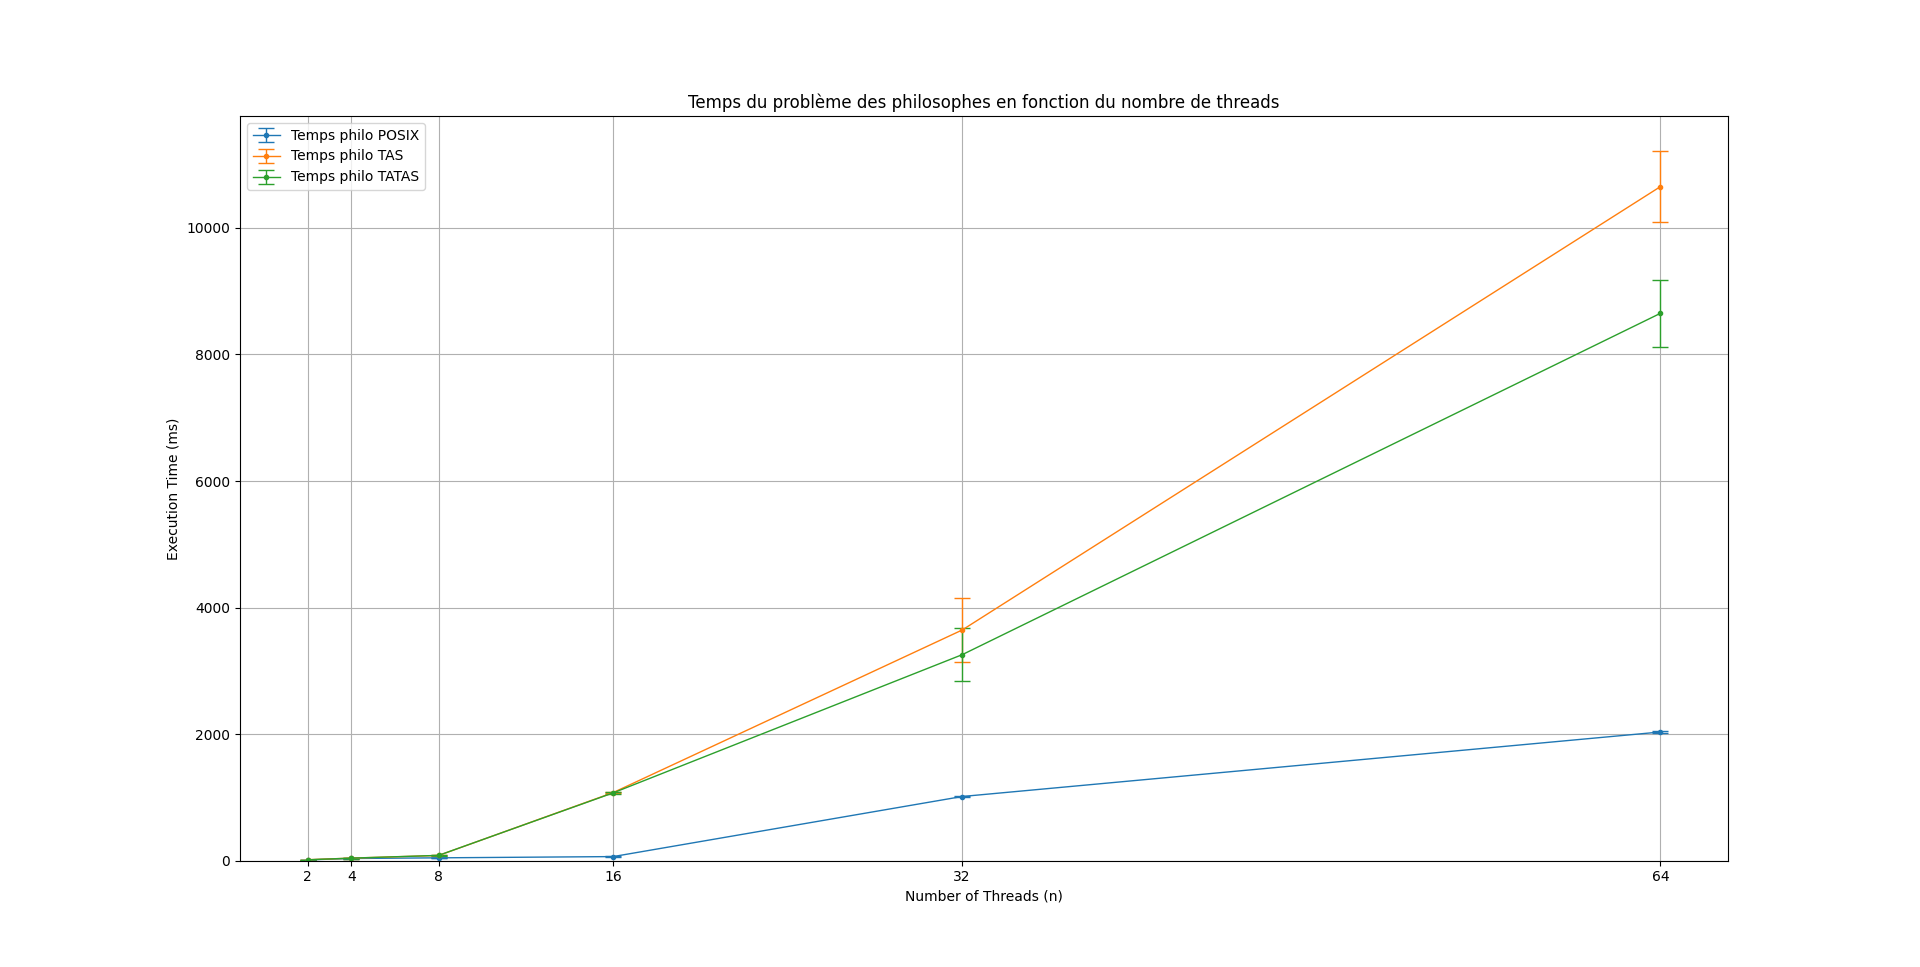
\includegraphics[width=\textwidth, keepaspectratio]{Temps_philo.png}
\centering
\end{figure}

L'analyse des résultats du problème des philosophes met en évidence une corrélation significative entre le temps d'exécution et le nombre de threads générés. Cette relation s'explique par la nature même du problème. Chaque thread, symbolisant un philosophe, bloque deux mutex, situés à sa droite et à sa gauche. Lorsqu'un thread voisin tente de verrouiller le mutex partagé, il doit attendre la libération de ce dernier. Avec une augmentation du nombre de threads, le nombre de ceux en attente croît proportionnellement. De plus, si le thread 1 bloque le mutex à sa gauche, le thread 2 bloque celui à sa gauche, et ainsi de suite, créant une séquence d'attentes entre les threads. Chaque thread doit patienter que son voisin libère le mutex à sa droite pour achever son exécution et libérer le mutex nécessaire à l'achèvement du thread suivant.

Cette observation souligne l'impact de la concurrence des threads sur le temps d'exécution du problème des philosophes. Une gestion efficace des ressources partagées et des mécanismes de synchronisation devient cruciale pour optimiser les performances de ce type d'application multi-threading.

De plus, on peut remarquer que les threads POSIX sont bien plus rapides que ceux utilisant l'algorithme test-and-set implémenté ou ceux utilisant l'algorithme test-and-test-and-set. Mais ceci est expliqué avec plus de détail dans la partie de l'implémentation de la synchronisation par attente active (voir section \ref{l'implémentation de la synchronisation par attente active}).

\subsection{Problème des Producteurs-Consommateurs}

\begin{figure}[H]
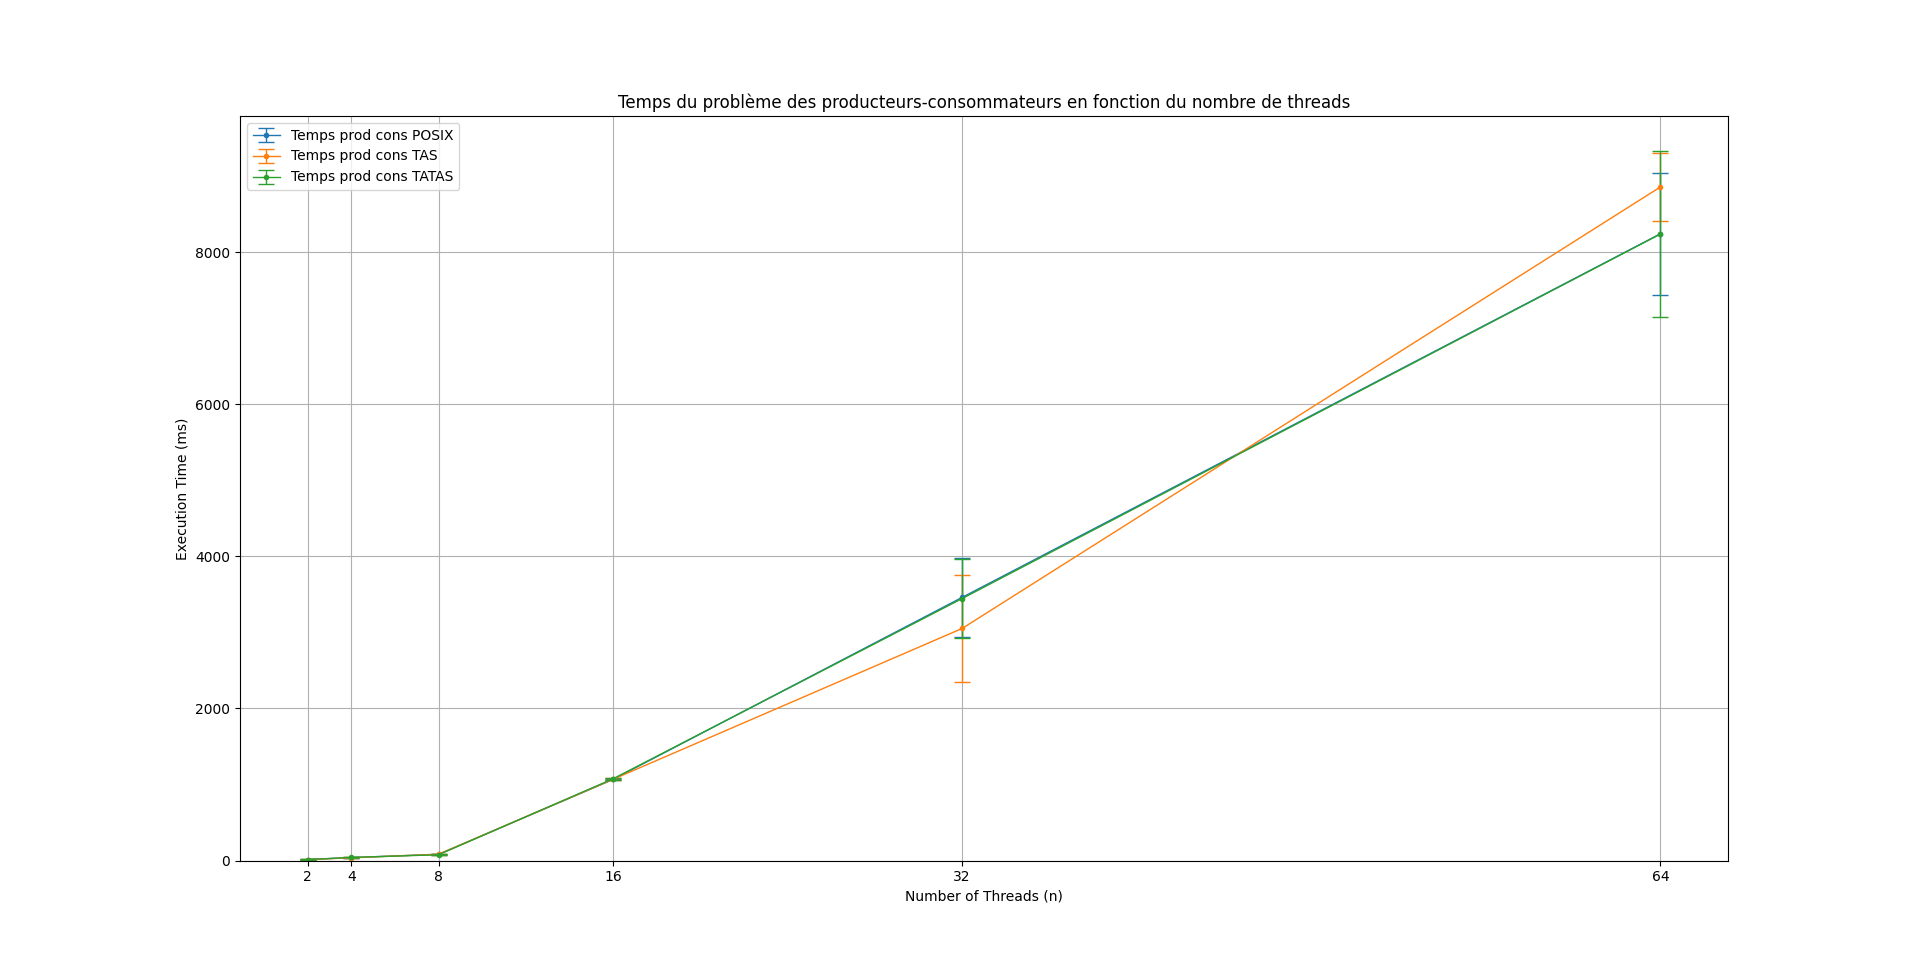
\includegraphics[width=\textwidth, keepaspectratio]{Temps_prod_cons.png}
\centering
\end{figure}

À la différence du problème des philosophes, le temps d'exécution du problème des producteurs-consommateurs augmente de manière constante avec le nombre de threads. L'utilisation des sémaphores permet une coordination efficace entre les threads, favorisant une conclusion plus rapide. Cette amélioration s'explique par la capacité des threads à travailler en collaboration, réduisant ainsi les conflits. En maintenant une gestion judicieuse des ressources partagées, notamment grâce aux sémaphores, les producteurs et les consommateurs peuvent opérer de manière plus harmonieuse. L'approche adoptée permet même aux consommateurs d'accéder à la ressource partagée même lorsque celle-ci n'est pas complètement remplie, évitant ainsi une perte de production.

\subsection{Problème des Lecteurs-Écrivains}

\begin{figure}[H]
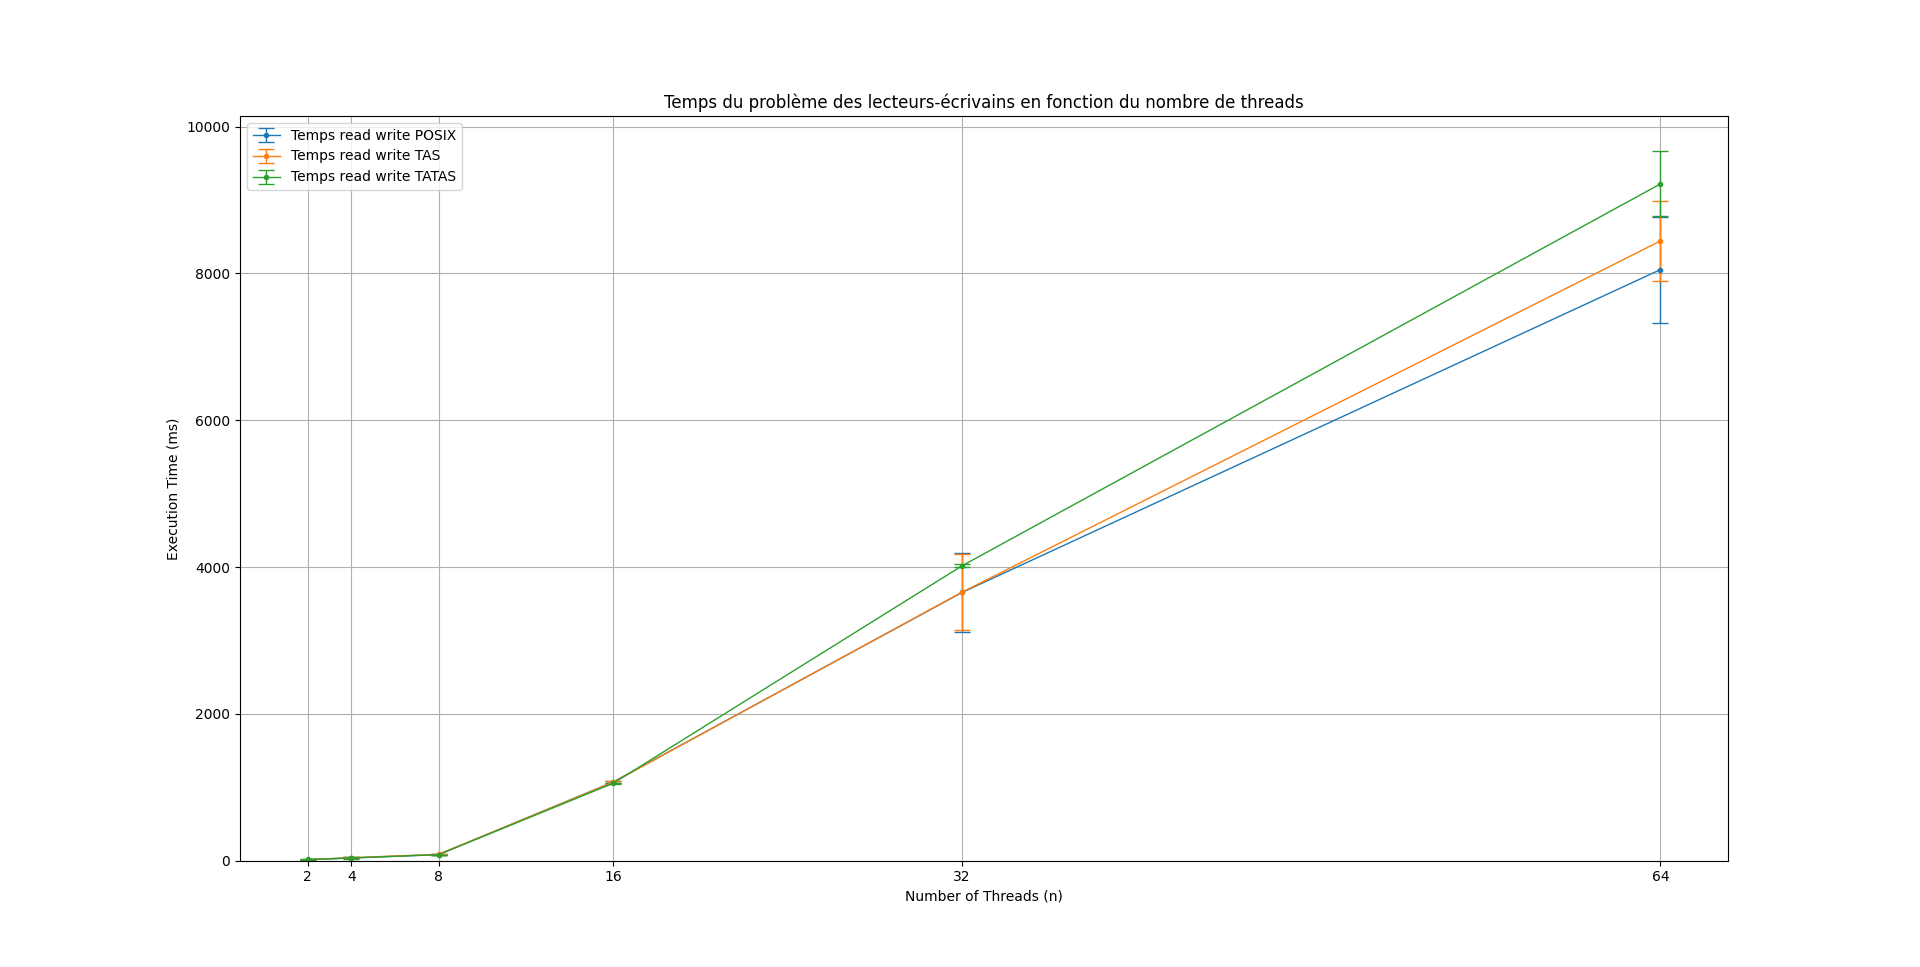
\includegraphics[width=\textwidth, keepaspectratio]{Temps_read_write.png}
\centering
\end{figure}

De manière similaire au problème des producteurs-consommateurs, le temps d'exécution du problème des lecteurs-écrivains augmente de manière constante avec le nombre de threads. La présence de mutexes assure l'absence de conflits entre lecteurs et écrivains, tandis que l'utilisation de sémaphores donne la priorité aux écrivains. Ainsi, lorsqu'un écrivain annonce son intention d'écrire, aucun lecteur ne peut accéder à la ressource partagée jusqu'à ce que le dernier lecteur libère cette ressource. Cette stratégie garantit l'intégrité des données partagées tout en permettant une gestion efficiente des accès concurrents.

\subsection{Implémentation de la Synchronisation par Attente Active}
\label{l'implémentation de la synchronisation par attente active}

\begin{figure}[H]
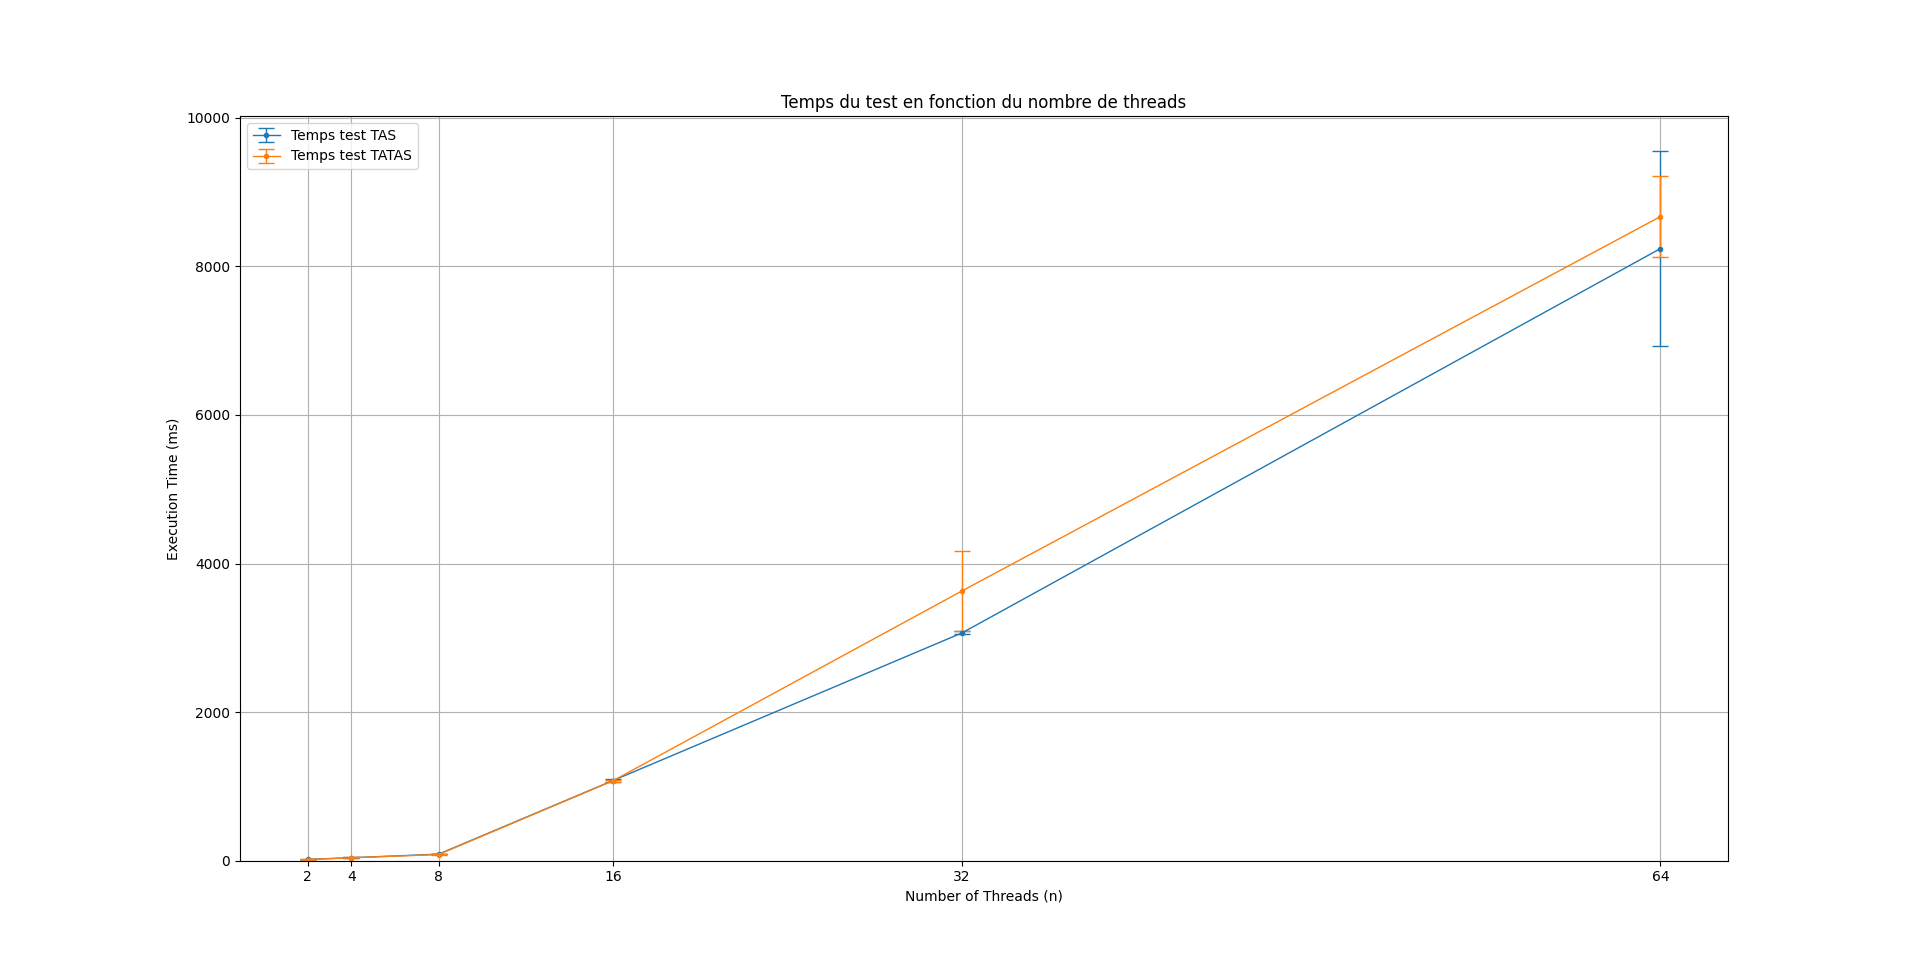
\includegraphics[width=\textwidth, keepaspectratio]{Temps_TAS_TATAS.png}
\centering
\end{figure}

Contrairement à ce qu'on pourrait penser en voyant le graphe, l'algorithme test-and-set (TAS) n'affiche pas une meilleure performance que test-and-test-and-set (TATAS). Les résultats indiquent une moyenne significativement inférieure pour TATAS par rapport à TAS. Cette disparité s'explique par le fonctionnement intrinsèque des deux algorithmes. TAS implique un nombre considérable d'opérations atomiques \emph{xchg}, lesquelles monopolisent les bus du CPU, entravant ainsi le lancement et l'achèvement des autres threads. En revanche, l'algorithme TATAS commence par une boucle de vérification de la disponibilité du verrou, n'effectuant une opération atomique \emph{xchg} qu'une fois cette condition remplie.

\section{Conclusion}

Ce projet a mis en lumière l'importance cruciale d'une gestion rigoureuse des conflits entre threads pour garantir le bon fonctionnement des programmes multi-threading. Les verrous se révèlent être des outils indispensables pour éviter des bugs sérieux, des programmes interminables, ou encore la perte de données critiques. Cependant, il est impératif de concevoir ces mécanismes avec précaution, car une implémentation maladroite peut non seulement ralentir considérablement un programme, mais aussi entraîner des dysfonctionnements majeurs, affectant même les performances globales du système.

\end{document}
